\documentclass[12pt,a4paper]{article}
\usepackage[UTF8]{ctex}
\usepackage{amsmath,amscd,amsbsy,amssymb,latexsym,url,bm,amsthm}
\usepackage{epsfig,graphicx,subfigure}
\usepackage{enumitem,balance}
\usepackage{wrapfig}
\usepackage{mathrsfs,euscript}
\usepackage[usenames]{xcolor}
\usepackage{hyperref}
\usepackage[vlined,ruled,linesnumbered]{algorithm2e}
\usepackage{float}
\usepackage{booktabs}
\usepackage{listings}
\usepackage{color}
\usepackage{caption}

\definecolor{mygreen}{rgb}{0,0.6,0}
\definecolor{mygray}{rgb}{0.5,0.5,0.5}
\definecolor{mymauve}{rgb}{0.58,0,0.82}
\lstset{
 backgroundcolor=\color{white}, 
 basicstyle = \footnotesize,       
 breakatwhitespace = false,        
 breaklines = true,                 
 captionpos = b,                    
 commentstyle = \color{mygreen}\bfseries,
 extendedchars = false,             
 frame =shadowbox, 
 framerule=0.5pt,
 keepspaces=true,
 keywordstyle=\color{blue}\bfseries, % keyword style
 language = Python,                     % the language of code
 otherkeywords={string}, 
 numbers=left, 
 numbersep=5pt,
 numberstyle=\tiny\color{mygray},
 rulecolor=\color{black},         
 showspaces=false,  
 showstringspaces=false, 
 showtabs=false,    
 stepnumber=1,         
 stringstyle=\color{mymauve},        % string literal style
 tabsize=4,          
 title=\lstname                      
}

\usepackage{fontspec}
\hypersetup{colorlinks=true,linkcolor=black}

\newtheorem{theorem}{Theorem}
\newtheorem{lemma}[theorem]{Lemma}
\newtheorem{proposition}[theorem]{Proposition}
\newtheorem{corollary}[theorem]{Corollary}
\newtheorem{exercise}{Exercise}
\newtheorem*{solution}{Solution}
\newtheorem{definition}{Definition}
\theoremstyle{definition}

\renewcommand{\thefootnote}{\fnsymbol{footnote}}

\newcommand{\postscript}[2]
 {\setlength{\epsfxsize}{#2\hsize}
  \centerline{\epsfbox{#1}}}

\renewcommand{\baselinestretch}{1.0}

\setlength{\oddsidemargin}{-0.365in}
\setlength{\evensidemargin}{-0.365in}
\setlength{\topmargin}{-0.3in}
\setlength{\headheight}{0in}
\setlength{\headsep}{0in}
\setlength{\textheight}{10.1in}
\setlength{\textwidth}{7in}
\makeatletter \renewenvironment{proof}[1][Proof] {\par\pushQED{\qed}\normalfont\topsep6\p@\@plus6\p@\relax\trivlist\item[\hskip\labelsep\bfseries#1\@addpunct{.}]\ignorespaces}{\popQED\endtrivlist\@endpefalse} \makeatother
\makeatletter
\renewenvironment{solution}[1][Solution] {\par\pushQED{\qed}\normalfont\topsep6\p@\@plus6\p@\relax\trivlist\item[\hskip\labelsep\bfseries#1\@addpunct{.}]\ignorespaces}{\popQED\endtrivlist\@endpefalse} \makeatother

\begin{document}
\noindent
\captionsetup[figure]{labelfont={bf},name={Fig.},labelsep=period}
\captionsetup[table]{labelfont={bf},name={Tab.},labelsep=period}
%========================================================================
\noindent\framebox[\linewidth]{\shortstack[c]{
\Large{\textbf{DCP3362 Computer Organization Lab01}}\vspace{1mm}\\
\footnotesize{\color{blue}$*$ Name: 石育瑋  \quad ID: A073708 \quad Email: stoneonetwo1203@gmail.com}}}

\section{Architecture diagrams}

\begin{figure}[H]
\centering
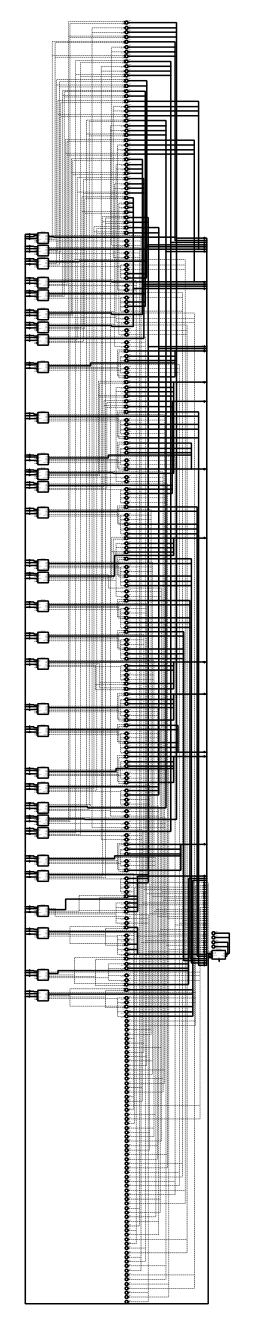
\includegraphics[height=21cm]{fig/alu.png}
\caption{alu模擬圖}
\label{fig:alu}
\end{figure}

\begin{figure}[H]
\centering
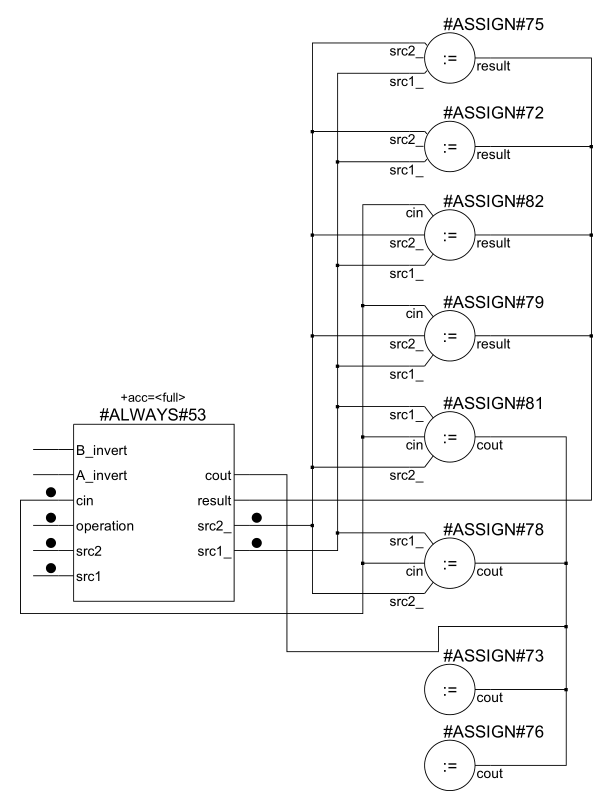
\includegraphics[height=6cm]{fig/alu_top.png}
\caption{alu$\_$top模擬圖}
\label{fig:alu_top}
\end{figure}


\section{Hardware module analysis}

\section{Experiment result}

實驗透過助教提供的Test Bench與ModelSim進行模擬測試,表\ref{tab:data}為輸入的測試數據表格,分別對6種不同的運算測驗,模擬出來得到的結果在表\ref{tab:result}中,最終結果正確無偏差。
\begin{table}[H]
\centering
\caption
{實驗數據}
\label{tab:data}
\begin{tabular}{llll} \toprule
operation & OP code & src1 & src2 \\
\midrule
AND & 0000 & ffff0000 & 0000ffff
\\
OR & 0001 & 3113c398 & 088e4954
\\
ADD & 0010 & ffffffff & 00000001
\\
SUB & 0110 & 7eda5023 & 2ec36ae5
\\
SLT & 0111 & ffffffff & 00000001
\\
NOR & 1100 & 00000000 & 00000000
\\ \bottomrule
\end{tabular}
\end{table}

\begin{table}[H]
\centering
\caption
{實驗結果}
\label{tab:result}
\begin{tabular}{ll} \toprule
Result & ZCV \\
\midrule
00000000 & 100
\\
399fcbdc & 000
\\
00000000 & 110
\\
5016e53e & 010
\\
00000001 & 000
\\
ffffffff & 000
\\ \bottomrule
\end{tabular}
\end{table}

\section{Problems you met and solutions}

在寫LAB時,主要有遇到以下幾個問題:
\begin{enumerate}
\item
\end{enumerate}

\section{Summary}



%========================================================================
\end{document}
